Zunächst wird die mittlere Weglänge der Elektronen mit Formel \eqref{eqn:wbar}
und \eqref{eqn:psat} berechnet. Die Ergebnisse werden dann mit dem Abstand $a$
zwischen Kathode und Beschleunigungselektrode verglichen. Der Abstand der
verwendeten Apparatur beträgt $a=1\,\cdot10^{-2}\mt$ \cite{601}.
\begin{table}
  \centering
  \begin{tabular}{ccc}
    \toprule
    $T/\Kel$ & $\bar w/\mt$ & $\frac{a}{\bar w}$ \\
    \midrule
     296.15 & $6.38\,\cdot 10^{-3}$ &    1.6  \\
     383.15 & $3.28\,\cdot 10^{-5}$ &  304.9  \\
     433.15 & $4.13\,\cdot 10^{-6}$ & 2421.3  \\
     443.15 & $2.89\,\cdot 10^{-6}$ & 3460.2  \\
    \bottomrule
  \end{tabular}
  \caption{Die mittlere Weglänge der Elektronen.}
  \label{tab:weg}
\end{table}

Die Frank-Hertz-Kurve des Hg-Dampfes ist in Abb. \ref{fig:kurve} zu sehen.
Dabei wird $U_\su{B}$ gegen $I_\su{A}$ geplottet.
\begin{figure}
  \centering
  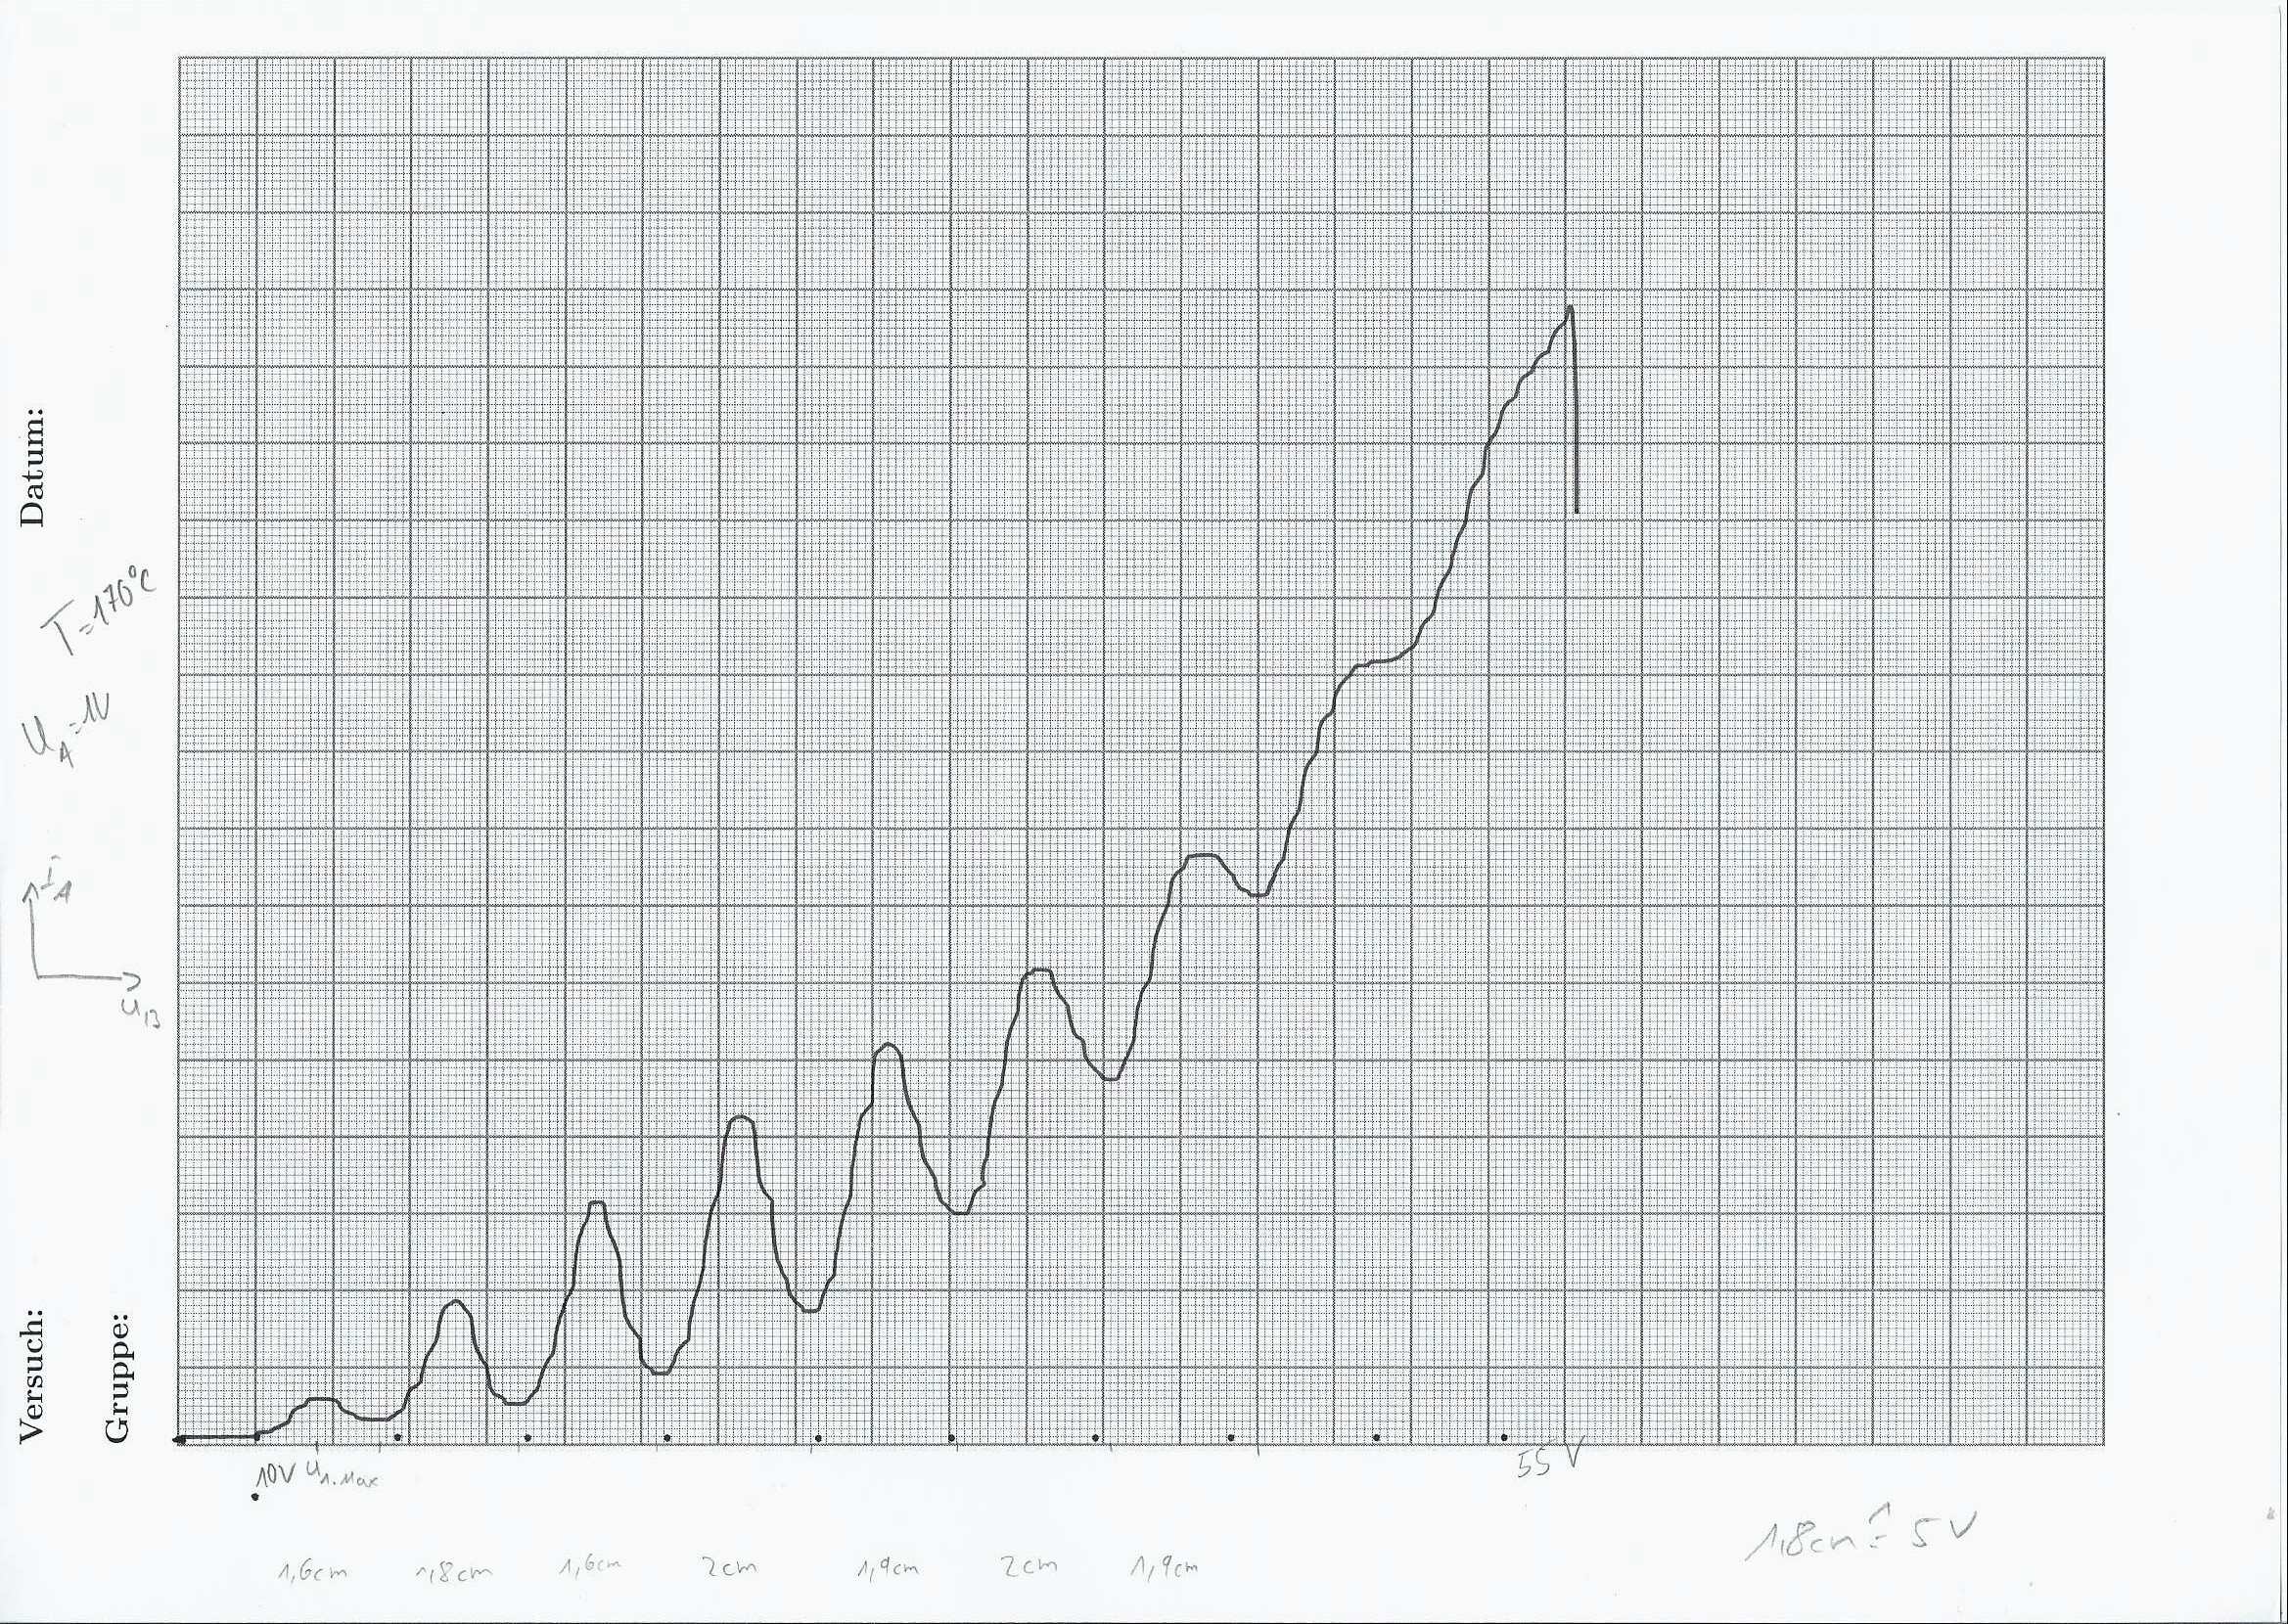
\includegraphics[width=0.8\textwidth]{bilder/kurve.jpg}
  \caption{Frank-Hertz-Kurve zu Hg-Dampf.}
  \label{fig:kurve}
\end{figure}
Die Temperatur wird auf $T=170\,\si{\degree}$ geregelt. Um die Anregungsenergien
$\Delta E$
des ersten Zustands von Hg zu bestimmen werden die Abstände der Maxima $\zeta$ in
$\cm$ gemessen. Anhand der Abbildung \ref{fig:kurve} lässt sich ermitteln,
dass $5\Volt = (1.8\pm0.2)\cm$ entsprechen. Die jeweiligen Werte für $\Delta U$
lassen sich dann bestimmen. Mit
\begin{equation}
  \Delta E = e\cdot \Delta U
\end{equation}
ergeben sich die entsprechenden Energien. Alle benötigten Werte sind in Tabelle
\ref{tab:werte} zu finden.
\begin{table}
  \centering
  \begin{tabular}{c c}
    \toprule
    $\zeta \,/\cm$   & $\Delta E \,/\eV$  \\
    \midrule
    1.6 & 4.44 \\
    1.8 & 5.00 \\
    1.6 & 4.44 \\
    2.0 & 5.56 \\
    1.9 & 5.28 \\
    \bottomrule
  \end{tabular}
  \caption{Abstände $\zeta$ und Anregungsenergien $\Delta E$ des ersten Anregungszustands.}
  \label{tab:werte}
\end{table}
Für $\zeta$ ergibt sich dann ein Mittelwert von
\begin{equation*}
  \zeta = (1.8\pm0.2)\cm
\end{equation*}
Für den Mittelwert folgt:
\begin{equation*}
  \Delta E = (4.9 \pm 0.4) \eV.
\end{equation*}
Mit
\begin{equation}
  \lambda = \frac{hc}{\Delta E} \label{eqn:lambda}
\end{equation}
lässt sich die Wellenlänge
\begin{equation*}
  \lambda = (250 \pm 20)\nm
\end{equation*}
mit der Gauß'schen Fehlerfortpflanzung
\begin{equation*}
  \Delta \lambda = \sqrt{\left(\frac{hc}{\DeltaE^2}\right)^2\cdot\sigma_\su{\Delta E^2}}
\end{equation*}
berechnen.

Das Kontaktpotential $K$ ergibt sich aus der Differenz der Spannungsdifferenz $\Delta U$
der Anregungsenergien für Quecksilber und der Spannung $U_\su{1.Max}$ bei dem das
erste Maximum auftritt. Es gilt $U_\su{1.Max} = 12.2\Volt$. Mit $\Delta U = 4.9\Volt$
folgt:
\begin{equation}
  K_1 = (7.3\pm0.2)\Volt.
\end{equation}
Der Fehler ergibt sich aus der Fehlerfortpflanzung
\begin{equation}
  \Delta k = \sqrt{\sigma_\su{U_B}}.
\end{equation}

Eine Weitere Möglichkeit zur Bestimmung des Kontaktpotentials ist mithilfe
des Plots \ref{fig:plot} gegeben.
\begin{figure}
  \centering
  \includegraphics[width=0.6\textwidth]{bilder/plt.pdf}
  \caption{Bestimmung des Kontaktpotentials über die Steigung $\sfrac{dI_\su{A}}{dU_\su{A}}$.}
  \label{fig:plot}
\end{figure}
Das Kontaktpotential $K$ ergibt sich dann aus der Beschleunigungsspannung minus
des Maximus des Graphen:
\begin{equation}
  K_2 = U_\su{B} - U_\su{max} = 13\Volt - 9.8\Volt = (3.2\pm0.2)\Volt.
\end{equation}
Damit ergibt sich für den Mittelwert des Kontaktpotentials
\begin{equation}
  \bar{K} = (5 \pm 2) \Volt.
\end{equation}

Zur Bestimmung der Ionisierungsenergie wird der Graph aus Abb. \ref{fig:ion}
verwendet.
\begin{figure}
  \centering
  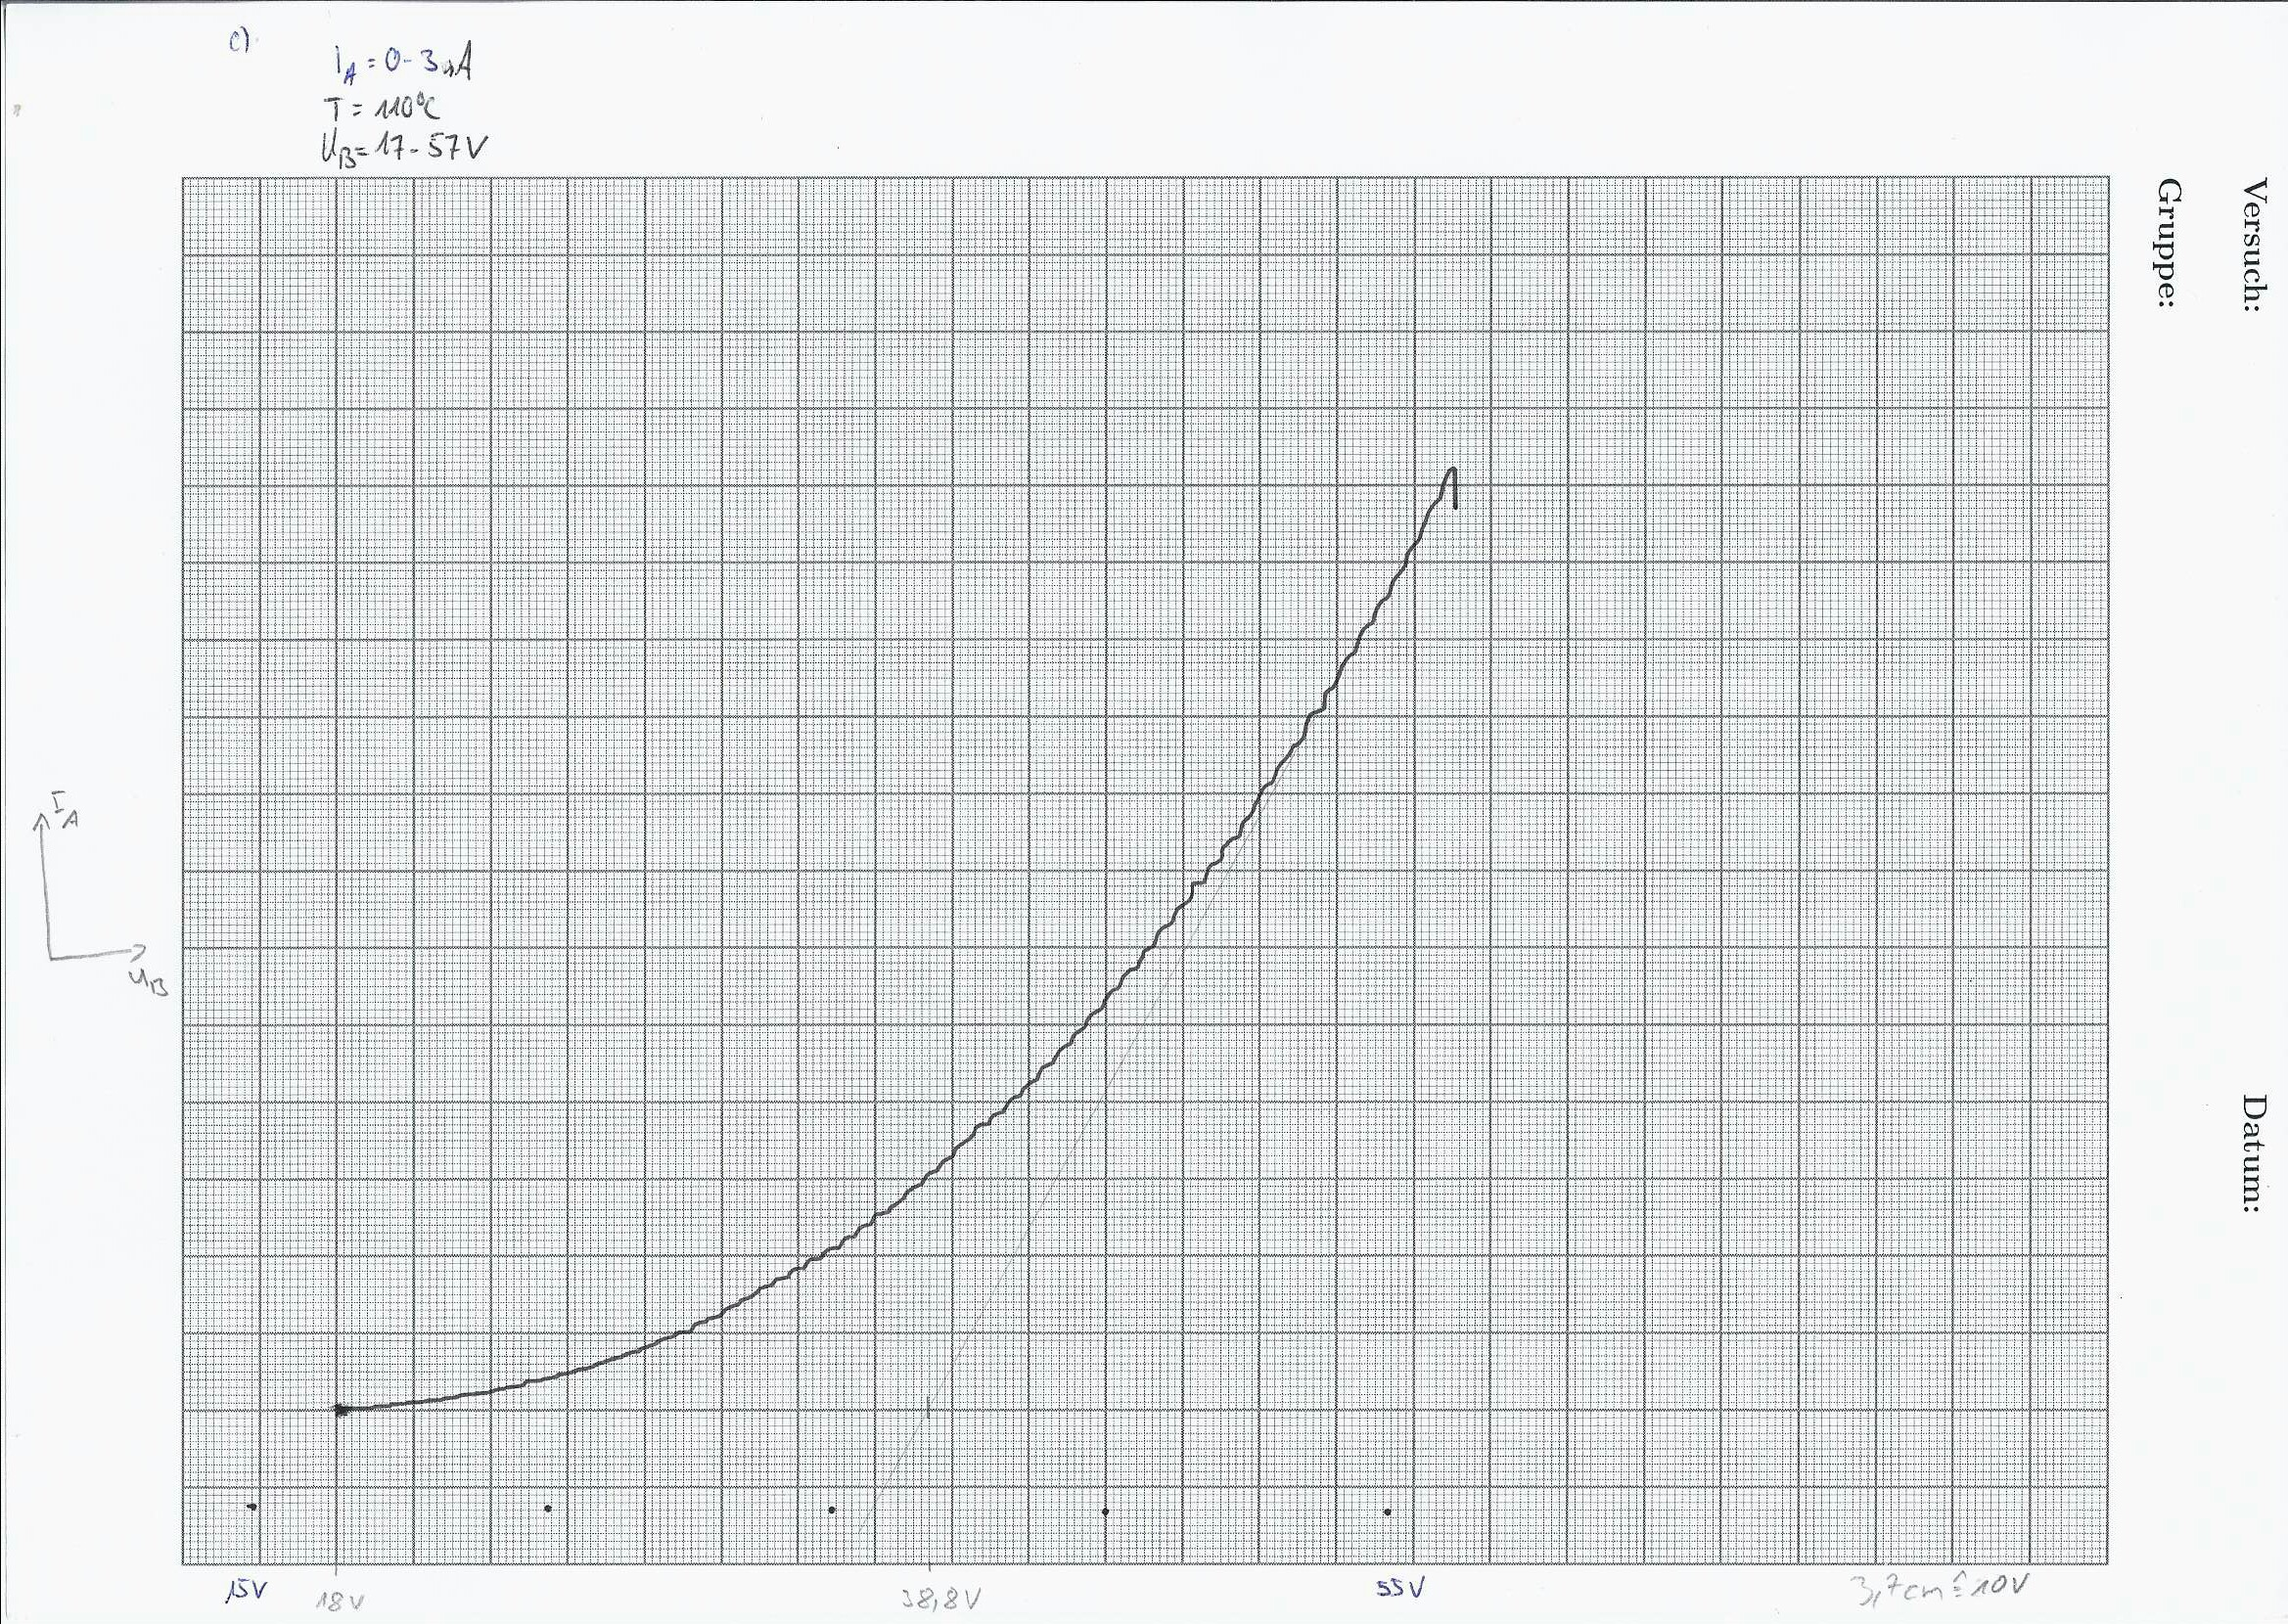
\includegraphics[width=0.8\textwidth]{bilder/ion.jpg}
  \caption{$I_\su{A}$ gegen $U_\su{B}$ zur Bestimmung der Ionisierungsenergie.}
  \label{fig:ion}
\end{figure}
Dazu wird versucht, eine Ausgleichsgerade einzuzeichnen, welche im Unendlichen starten
soll. Im Idealfall wäre dies eine Asymptote, das ist jedoch bei diesem Graphen nicht
der Fall. Der Schnittpunkt mit der x-Achse liegt bei $U_\su{x} = 38.8 \Volt$.
Die Ionisierungsenergie ergibt sich dann, indem das Kontaktpotential $K$ von
dem Schnittpunkt abgezogen wird.
\begin{equation}
  E_\su{ion} = (U_\su{x}-\bar{K}) \cdot e = 33.8\eV
\end{equation}
